\documentclass[border=8pt]{standalone}
\usepackage{fontspec}
\setsansfont{Arial}
\usepackage{pgfplots}
\pgfplotsset{compat=1.18,
  every axis/.append style={/pgf/number format/assume math mode=true,
    tick label style={font=\sffamily\small},
    nodes near coords style={font=\sffamily\scriptsize}}}
% Validation versus published-test AP@[.50:.95] (%) for the frozen T41 pair.
% Source: docs/t41-results.md, Results table (PR #25).
\begin{document}
\sffamily\small
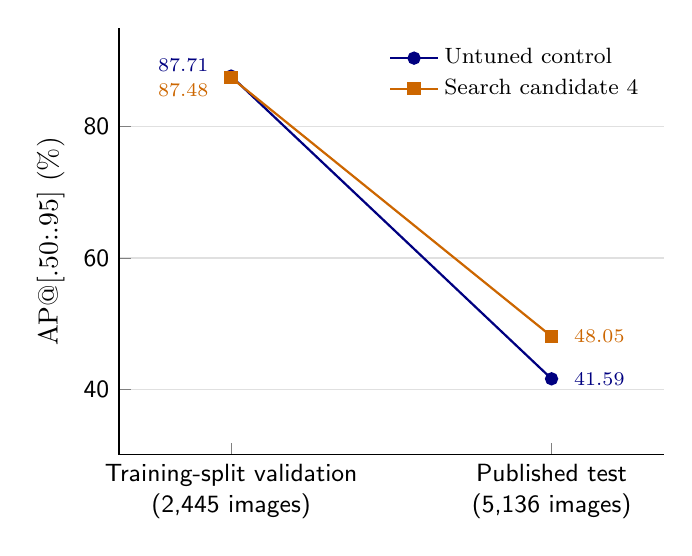
\begin{tikzpicture}
\begin{axis}[
  width=8.5cm,height=7cm,
  xmin=-0.35,xmax=1.35,ymin=30,ymax=95,
  xtick={0,1},
  xticklabels={{Training-split validation\\(2{,}445 images)},{Published test\\(5{,}136 images)}},
  xticklabel style={align=center},
  ylabel={AP@[.50:.95] (\%)},
  ymajorgrids,grid style={black!12},
  axis lines*=left,
  legend style={font=\footnotesize,draw=none,fill=none,at={(0.98,0.98)},anchor=north east},
  legend cell align=left,
]
\addplot[blue!50!black,thick,mark=*] coordinates {(0,87.7062) (1,41.5886)};
\addplot[orange!80!black,thick,mark=square*] coordinates {(0,87.4833) (1,48.0502)};
\node[font=\scriptsize,anchor=east,blue!50!black] at (axis cs:-0.04,89.4) {87.71};
\node[font=\scriptsize,anchor=east,orange!80!black] at (axis cs:-0.04,85.6) {87.48};
\node[font=\scriptsize,anchor=west,blue!50!black] at (axis cs:1.04,41.59) {41.59};
\node[font=\scriptsize,anchor=west,orange!80!black] at (axis cs:1.04,48.05) {48.05};
\legend{Untuned control,Search candidate 4}
\end{axis}
\end{tikzpicture}
\end{document}
